\documentclass[conference]{IEEEtran}

\usepackage[utf8]{inputenc}
\usepackage[spanish,es-noshorthands]{babel}
\usepackage{amsmath}
\usepackage{graphicx}
\usepackage{subcaption}
\usepackage{booktabs}
\usepackage{array}
\usepackage{url}
\usepackage{listings}

\addto\captionsspanish{\renewcommand{\tablename}{Tabla}%
\renewcommand{\figurename}{Fig.}}
\renewcommand{\IEEEkeywordsname}{Palabras clave}
\renewcommand{\refname}{Referencias}

\urlstyle{same}

% El entorno de compilación no incluye las fuentes Times (ptm/psnfss).
% Se conserva la clase IEEEtran y se sustituye la familia por Computer Modern.
\renewcommand{\rmdefault}{cmr}
\renewcommand{\sfdefault}{cmss}
\renewcommand{\ttdefault}{cmtt}
\makeatletter
\gdef\@IEEESAVESTATEfontfamily{cmr}
\makeatother

\lstset{
  basicstyle=\ttfamily\scriptsize,
  breaklines=true,
  columns=fullflexible,
  keepspaces=true,
  frame=single,
  extendedchars=true,
  inputencoding=utf8,
  literate={á}{{\'a}}1 {é}{{\'e}}1 {í}{{\'i}}1 {ó}{{\'o}}1 {ú}{{\'u}}1
           {Á}{{\'A}}1 {É}{{\'E}}1 {Í}{{\'I}}1 {Ó}{{\'O}}1 {Ú}{{\'U}}1
           {ñ}{{\~n}}1 {Ñ}{{\~N}}1 {ü}{{\"u}}1
}
\renewcommand{\lstlistingname}{Listado}

\begin{document}

\title{Documentación de la migración de JavaScript a TypeScript en la
aplicación web \emph{Finanzas del hogar}}

\author{
  \IEEEauthorblockN{Juan Carlos Merchan}
  \IEEEauthorblockA{Universidad --- Electiva 2 -- Desarrollo Web\\
  09/11/2026\\
  \texttt{autor@dominio}}
}

\maketitle

\begin{abstract}
Se documenta la migración de una aplicación web monolítica de gestión
financiera del hogar, construida con Express, EJS y MongoDB, desde JavaScript con módulos
ECMAScript hacia TypeScript estricto. El proceso conservó el comportamiento
funcional y adoptó programación orientada a objetos en los modelos de datos,
mediante interfaces y clases. El esquema de verificación combinó el compilador
de TypeScript con pruebas funcionales de extremo a extremo: el árbol migrado pasó de 686 a 0 errores de
\texttt{tsc --noEmit} y superó 204 de 204 comprobaciones funcionales. El
artículo describe el contexto del sistema original, la metodología por capas,
la arquitectura resultante, cinco diagramas del Lenguaje Unificado de
Modelado (UML) y las lecciones aprendidas. Su
enfoque es documental: no se rehace la migración ni se propone una
reingeniería.
\end{abstract}

\begin{IEEEkeywords}
migración de software, TypeScript, Express, Mongoose, UML, verificación
\end{IEEEkeywords}

\section{Introducción}

\subsection{Contexto y problema}
La aplicación web \emph{Finanzas del hogar} es un proyecto académico de la
asignatura Electiva 2 -- Desarrollo Web. Permite administrar hogares, cuentas,
transacciones de ingreso y gasto, categorías, presupuestos y reportes. El
sistema se implementó originalmente como un monolito JavaScript ESM sobre
Express, con vistas EJS y persistencia en MongoDB mediante Mongoose. Aunque el
código funcionaba, la ausencia de tipos hacía que los contratos entre capas
existieran solo en la documentación y en la memoria del autor: los cuerpos de
petición llegaban como objetos sin forma declarada, los servicios aceptaban y
devolvían estructuras verificadas únicamente en tiempo de ejecución y
cualquier refactorización exigía recorrer manualmente los puntos de uso. El
problema documentado no fue un fallo funcional, sino un costo estructural de
mantenimiento y una barrera para demostrar corrección.\footnote{La plantilla
IEEEtran fue adaptada localmente para usar Computer Modern; consúltese
\texttt{README\_compilacion.txt}.}

\subsection{Objetivo y alcance}
El objetivo es documentar, con evidencia verificable, la migración de ese
monolito a TypeScript estricto, sin rehacerla y sin alterar el comportamiento
observable. El alcance comprende el backend de 53 archivos, las dos fuentes
del frontend y los artefactos generados que se publican con el sitio. Quedan
fuera del proceso migratorio las funcionalidades incorporadas después del
cierre de la migración, que se describen como estado actual en la Sección IV y
se delimitan en la Sección VI. El correo del autor se conserva como marcador
explícito\footnote{Dato pendiente de completar.}.

\subsection{Aportes}
El artículo ofrece tres aportes. Primero, una descripción ordenada de la
migración por capas, con las decisiones que permitieron pasar de un árbol sin
tipos a uno estrictamente verificado. Segundo, la formalización del patrón de
programación orientada a objetos aplicado a los modelos de Mongoose, incluida
la distinción entre interfaz de contrato y clase de estáticos. Tercero, un
protocolo de verificación reproducible (686 a 0 errores, 204/204
comprobaciones) y trazabilidad de snapshots por commit
(\texttt{fb1ad1d} a \texttt{34016bd}).

\subsection{Organización}
La Sección II describe el sistema original en JavaScript. La Sección III
presenta la metodología y el proceso de migración. La Sección IV caracteriza
la arquitectura del sistema migrado en su estado actual. La Sección V explica
los cinco diagramas UML. La Sección VI reúne resultados, validación y lecciones
aprendidas. La Sección VII formula las conclusiones y la Sección VIII lista las
referencias.

\section{Contexto del sistema original en JavaScript}

\subsection{Descripción funcional}
El sistema organiza la información financiera por hogar. Cada hogar agrupa
miembros con rol de administrador o miembro, y delimita cuentas, categorías de
ingreso y gasto, transacciones, presupuestos mensuales y reportes. La
autenticación se resuelve con sesiones basadas en JSON Web Tokens almacenados
en cookies, y la documentación de la interfaz de programación se publica con
Swagger. La aplicación expone dos superficies: rutas web que renderizan vistas
EJS y rutas de interfaz de programación que responden JSON.

\subsection{Stack tecnológico original}
La Tabla~\ref{tab:stack} resume las tecnologías declaradas en el momento de la
migración. Las versiones corresponden a los rangos del archivo
\texttt{package.json} en el commit \texttt{34016bd}; no se presentan versiones
instaladas ni el estado actual de las dependencias.

\begin{table}[!t]
\caption{Stack declarado al momento de la migración (commit \texttt{34016bd})}
\label{tab:stack}
\centering
\footnotesize
\begin{tabular}{@{}>{\raggedright\arraybackslash}p{2.05cm}>{\raggedright\arraybackslash}p{2.05cm}>{\raggedright\arraybackslash}p{1.4cm}>{\raggedright\arraybackslash}p{2.1cm}@{}}
\toprule
Componente & Tecnología & Versión & Evidencia \\
\midrule
Servidor HTTP & Express & \textasciicircum{}5.2.1 & \texttt{package.json} \\
Vistas & EJS & \textasciicircum{}7.0.1 & \texttt{package.json} \\
Persistencia & Mongoose & \textasciicircum{}9.11.0 & \texttt{package.json} \\
Autenticación & jsonwebtoken & \textasciicircum{}9.0.3 & \texttt{package.json} \\
Documentación & swagger-jsdoc & \textasciicircum{}6.3.0 & \texttt{package.json} \\
Configuración & dotenv & \textasciicircum{}18.0.5 & \texttt{package.json} \\
Runtime & Node.js ESM & no disponible & \texttt{package.json} \\
Ejecución TS & tsx & \textasciicircum{}4.23.15 & \texttt{package.json} \\
Compilador & TypeScript & \textasciicircum{}7.0.2 & \texttt{package.json} \\
Bundler & esbuild & \textasciicircum{}0.28.2 & \texttt{package.json} \\
\bottomrule
\end{tabular}
\end{table}

\subsection{Organización del código}
El backend se organizaba en carpetas técnicas: \texttt{config},
\texttt{controllers}, \texttt{driver}, \texttt{middlewares}, \texttt{models},
\texttt{routes}, \texttt{services}, \texttt{types}, \texttt{utils} y
\texttt{views}. Los controladores se dividían en web y de interfaz de
programación; los servicios concentraban las reglas de negocio y los modelos
la definición de esquemas. La migración abarcó 53 archivos del backend y dos
fuentes del frontend, sin introducir una nueva capa arquitectónica.

\subsection{Limitaciones del JavaScript sin tipos}
La ausencia de anotaciones no impedía operar el sistema, pero trasladaba la
verificación al tiempo de ejecución. Los errores de forma en un cuerpo de
petición se descubrían al responder una solicitud, no al compilar. Los
contratos de los servicios dependían de convenciones y los cambios de firma
podían propagarse sin aviso hasta un punto de uso lejano. A ello se sumaba la
documentación OpenAPI \cite{openapi}, que describía la interfaz pero no
obligaba al código a respetarla.

\subsection{Estado de partida}
El punto de partida de la migración se fijó con la cifra de 686 errores de
\texttt{tsc --noEmit} sobre el árbol recién renombrado. Es decir, no se trata
de 686 defectos funcionales, sino del total de diagnósticos emitidos por el
compilador al activar la verificación estricta sobre los archivos que antes se
ejecutaban como JavaScript. Ese valor operó como línea base y como criterio de
avance: cada capa se consideraba terminada cuando reducía el conteo sin
introducir cambios de comportamiento. El detalle del estado inicial se
conserva en el snapshot del commit \texttt{fb1ad1d} (Anexo A.2).

\section{Metodología y proceso de migración}

\subsection{Estrategia general}
La migración se planteó como una transformación de tipos, no como una
reescritura. Se preservaron las rutas, los códigos HTTP, los textos de
respuesta y los flujos de error. La verificación se separó de la ejecución: el
compilador se ejecuta con \texttt{tsc --noEmit} y el servidor se inicia con
\texttt{tsx} \cite{tsx}, que transpila en caliente sin generar un directorio
de distribución. Esta separación evitó un paso de compilación en el despliegue y
permitió tratar el tipado como una propiedad verificable del repositorio.

\subsection{Renombrado mecánico}
La primera fase fue deliberadamente mecánica. Se renombraron 53 archivos
\texttt{.mjs} a \texttt{.ts} conservando el historial de git, se sustituyeron
106 especificadores de importación para que apuntaran a la nueva extensión y
se actualizaron los patrones de \texttt{swagger-jsdoc} que alimentan el
documento OpenAPI. La fase se cerró con dos comprobaciones negativas: ninguna
extensión \texttt{.mjs} permanecía en \texttt{src/} y ninguna referencia a
\texttt{.mjs} sobrevivía en el código.

\subsection{Configuración del compilador}
La configuración adoptada se reproduce en el Listado~\ref{lst:tsconfig}.\footnote{Archivo
no incluido en los ocho snapshots de A.2; se cita desde el commit
\texttt{34016bd}.} Su propósito es demostrar que la verificación estricta se
aplicó a todo el árbol,
incluido el frontend, y que el compilador se usó sin emitir archivos.

\begin{lstlisting}[caption={Configuración del compilador (\texttt{tsconfig.json})},
label={lst:tsconfig}]
{
  "compilerOptions": {
    "target": "ES2022",
    "module": "nodenext",
    "moduleResolution": "nodenext",
    "lib": ["ES2022", "DOM", "DOM.Iterable"],
    "types": ["node"],
    "strict": true,
    "noEmit": true,
    "allowImportingTsExtensions": true,
    "verbatimModuleSyntax": true,
    "isolatedModules": true,
    "esModuleInterop": true,
    "skipLibCheck": true
  },
  "include": ["src"]
}
\end{lstlisting}

Tres decisiones explican el resultado. \texttt{strict} activa el conjunto
completo de comprobaciones \cite{typescript-handbook,tsconfig-strict};
\texttt{verbatimModuleSyntax} obliga a declarar con \texttt{import type} los
imports que solo aportan tipos; y \texttt{allowImportingTsExtensions} permite
que los imports internos lleven la extensión \texttt{.ts}, coherente con el
modo ESM y con \texttt{tsx}. La opción \texttt{lib} incluye el DOM porque las
fuentes del frontend viven bajo \texttt{src/} y se validan en la misma
ejecución. La configuración completa se conserva en el commit \texttt{34016bd}; no forma parte de los ocho archivos representativos del Anexo A.2.

\subsection{Orden de migración por capas}
La migración avanzó de abajo hacia arriba, con el compilador como puerta de
cada etapa: configuración, utilidades y driver; middlewares; modelos;
servicios; controladores y, finalmente, el punto de entrada. El orden no fue
arbitrario: cada capa dependía de contratos ya estabilizados en la anterior,
de modo que los errores restantes señalaban deuda localizada y no ruido
cruzado. Los servicios recibieron los cuerpos de petición como
\texttt{unknown} y los transformaron en estructuras limpias antes de persistir;
los controladores se anotaron como manejadores de Express; y el punto de
entrada se tipó junto con la corrección de una doble invocación de arranque.

\subsection{Programación orientada a objetos en los modelos}
El hallazgo técnico más relevante fue que \texttt{Model} de Mongoose se declara
como interfaz, no como clase. Extender una clase desde esa interfaz colapsa los
miembros heredados a \texttt{any} y anula el chequeo. El patrón adoptado separa
tres piezas: la interfaz del documento, la interfaz del contrato del modelo y
una clase que implementa los estáticos y se copia al esquema con
\texttt{loadClass} \cite{mongoose-model}. El Listado~\ref{lst:modelo} reproduce
la aplicación del patrón al modelo de usuario.

\begin{lstlisting}[caption={Contrato de modelo y estáticos copiados con \texttt{loadClass}},
label={lst:modelo}]
export interface IUserModel extends Model<IUser> {
  findByEmail(email: string): Promise<IUser | null>;
  findLeanById(userId: Types.ObjectId | string): Promise<IUser | null>;
}

class UserModel extends Model<IUser> {
  static findByEmail(this: IUserModel, email: string) {
    return this.findOne({ email: email.trim().toLowerCase() }).lean();
  }
}

userSchema.loadClass(UserModel);
export const User = mongoose.model<IUser, IUserModel>('User', userSchema);
\end{lstlisting}

El patrón se aplicó a siete modelos y se acompañó de enumeraciones con valores
idénticos a los almacenados, de modo que la validación de los esquemas no
cambiara. Los estáticos de dominio, como la búsqueda por correo o la
verificación de pertenencia al hogar, quedaron expuestos en el contrato y los
servicios los consumieron en lugar de construir filtros manuales. La versión completa de \texttt{src/models/user.ts} se conserva en el snapshot del Anexo A.2.

\subsection{Contratos de petición y augmentación de Express}
Las propiedades que los middlewares inyectan en la petición se declararon
mediante augmentación de tipos, como muestra el
Listado~\ref{lst:express}.\footnote{Archivo no incluido en los ocho snapshots
de A.2; se cita desde el commit \texttt{34016bd}.} Esto convierte el acceso a
\texttt{req.home} o \texttt{req.user} en una operación verificada y obliga a
resolver la posibilidad de que no existan.

\begin{lstlisting}[caption={Augmentación de \texttt{Express.Request}},
label={lst:express}]
declare global {
  namespace Express {
    interface Request {
      user?: IUser;
      home?: IHome;
      homeId?: string;
      homeRole?: Role;
    }
  }
}
\end{lstlisting}

En las rutas protegidas, los middlewares garantizan la presencia de esas
propiedades; por eso se empleó la aserción de no nulidad en lugar de añadir
guardas que habrían alterado los flujos de error. La aserción es una operación
de tipo y no modifica el valor en tiempo de ejecución. La declaración completa se conserva en el commit \texttt{34016bd}; su uso se evidencia en el snapshot de \texttt{src/middlewares/home.ts} del Anexo A.2.

\subsection{Errores y conversiones de tipo}
El compilador tipa el parámetro de \texttt{catch} como \texttt{unknown}. Para
no perder el chequeo estricto se introdujo un guardia
\texttt{isHttpError} y se reescribieron 31 condiciones de estado, de modo que
cada rama estrecha el tipo antes de leer el mensaje o los detalles. Las
conversiones se limitaron a operaciones de tipo: nunca transforman el valor en
tiempo de ejecución. Entre los ajustes puntuales figuran el paso de
\texttt{req.params} a cadenas tipadas, la aritmética de fechas mediante
\texttt{getTime} y el tratamiento de cargas JWT que pueden ser cadenas. Con
ello se corrigieron dos riesgos latentes sin cambiar respuestas: el acceso a
propiedades de una cadena y la aritmética implícita entre fechas.

\subsection{Frontend en TypeScript}
Las dos fuentes del frontend se trasladaron a \texttt{src/frontend} y se
compilaron con esbuild hacia \texttt{public/js} \cite{esbuild}. Los artefactos
generados se conservan en el repositorio porque el despliegue no ejecuta un
paso de compilación. Se mantuvieron las funciones autoejecutables, de modo que
el bundle no introduce módulos ni imports en tiempo de ejecución. La validación
de formularios y el gráfico del panel usan tipos del DOM y un contrato mínimo
para la biblioteca de gráficos, sin dependencias adicionales.

\subsection{Verificación}
La Tabla~\ref{tab:verificacion} reúne exclusivamente las cifras del momento
migratorio. El typecheck pasó de 686 a 0 errores y las suites HTTP quedaron en
204 comprobaciones exitosas sobre 204. Las cifras actuales del repositorio no
se incluyen en esta tabla porque corresponden a etapas posteriores.

\begin{table}[!t]
\caption{Verificación al cierre de la migración (commit \texttt{34016bd})}
\label{tab:verificacion}
\centering
\small
\begin{tabular}{@{}lcc@{}}
\toprule
Suite & Comprobaciones & Estado \\
\midrule
Estado base (\texttt{setup}) & --- & correcto \\
Transacciones (\texttt{i4}) & 52 & 52/52 \\
Presupuestos y permisos (\texttt{i5}) & 62 & 62/62 \\
Reportes y recursos (\texttt{i6}) & 49 & 49/49 \\
Autenticación y API (\texttt{i7smoke}) & 41 & 41/41 \\
\midrule
Total & 204 & 204/204 \\
\bottomrule
\end{tabular}

\vspace{2pt}
{\footnotesize Fuente: suites HTTP ejecutadas sobre el commit
\texttt{34016bd} (05/11/2026).}
\end{table}

Además del conteo, se comprobaron regresiones puntuales: la documentación
OpenAPI respondió con el documento generado y sus recursos, las rutas de
archivos estáticos sirvieron los bundles del frontend y los mensajes de sesión
se conservaron. El criterio de cierre fue doble: compilador sin errores y
suites sin fallos. La fuente de la Tabla~\ref{tab:verificacion} es la sección 9
del documento de migración incluido en el commit \texttt{34016bd}.

\subsection{Decisiones y alternativas descartadas}
Las alternativas evaluadas y su motivo de descarte se resumen en el Anexo A.1;
ninguna de ellas forma parte del flujo final.

\subsection{Trazabilidad de snapshots}
El índice de snapshots deja constancia del criterio de comparación, que se cita
textualmente:

\begin{quote}
\itshape
Los archivos de \texttt{antes/} provienen del commit \texttt{fb1ad1d}, estado
previo a la migración. Los de \texttt{despues/} provienen del commit
\texttt{34016bd} (``Migración completa a TypeScript estricto''), que cierra la
migración, y no de \texttt{HEAD}. El estado actual del repositorio puede
diferir de estos snapshots por las fases posteriores A--E.
\end{quote}

De acuerdo con esa nota, el estado actual del repositorio puede diferir por las
fases A--E posteriores; este artículo no las documenta como parte del proceso
migratorio. La comparación entre ambos commits se reproduce en el Anexo A.2.

\section{Arquitectura y diseño del sistema migrado}

Esta sección describe la arquitectura en el estado actual del repositorio y no
en el instante de cierre de la migración. Esa distinción es necesaria porque las
fases posteriores añadieron funcionalidad sobre la base ya tipada, sin alterar
la organización por capas que dejó el proceso migratorio.

\subsection{Estado actual y métricas}

El estado actual se fijó en el commit \texttt{cebc62a} (08/11/2026), posterior
al cierre migratorio de \texttt{34016bd} (05/11/2026). La
Tabla~\ref{tab:actual} resume el tamaño del árbol y declara la fuente de cada
cifra, de modo que las métricas puedan reconstruirse desde el historial. Las
cifras de esta tabla describen el repositorio completo y no se comparan con las
de la Tabla~\ref{tab:stack}, que consigna el stack declarado en el commit de
cierre de la migración.

\begin{table}[!t]
\caption{Dimensiones del repositorio en el estado actual (commit \texttt{cebc62a}, 08/11/2026)}
\label{tab:actual}
\centering
\small
\begin{tabular}{@{}lcc@{}}
\toprule
Categoría & Cantidad & Fuente \\
\midrule
Archivos TypeScript en \texttt{src/} & 67 & \texttt{git ls-files} \\
Vistas EJS & 24 & \texttt{src/views} \\
Modelos Mongoose & 9 & \texttt{src/models} \\
Controladores & 21 & \texttt{src/controllers} \\
Servicios & 11 & \texttt{src/services} \\
Archivos de rutas & 11 & \texttt{src/routes} \\
\bottomrule
\end{tabular}

\vspace{2pt}
{\footnotesize Fuente: repositorio en \texttt{cebc62a} (HEAD al 08/11/2026).}
\end{table}

\subsection{Capas y flujo de una petición}

El punto de entrada es \texttt{src/app.ts}. Allí se configura el motor de
vistas EJS, el middleware de diseño, los analizadores de cuerpo, la lectura de
cookies, los archivos estáticos y la autenticación. Después se registra un
middleware que carga en \texttt{res.locals} los datos comunes de la navegación
y, por último, se montan las superficies de la aplicación. El orden importa:
las rutas de interfaz de programación y de salud se resuelven antes del
middleware de locales para no ejecutar consultas innecesarias, y los
manejadores de error se registran al final.

Una petición recorre cinco puntos: ruta, middleware, controlador, servicio y
modelo. La ruta declara el verbo y la ruta; el middleware valida sesión, hogar
y rol; el controlador traduce la petición a una llamada de servicio; el
servicio aplica las reglas de negocio y consulta los modelos; y el modelo
persiste en MongoDB a través del controlador de base de datos. Las respuestas
web renderizan una vista EJS y las respuestas de interfaz de programación
devuelven JSON. Los errores ascienden por la cadena y los centraliza el
middleware de error, que distingue entre \texttt{HttpError} y fallos no
previstos.

\subsection{Configuración y arranque}

La configuración se concentra en \texttt{src/config}. El módulo de entorno lee
y valida las variables necesarias; el de base de datos establece la conexión;
el de Swagger compone el documento OpenAPI; y el de monedas fija los símbolos y
la precisión. El arranque se encapsula en una función asíncrona que primero
conecta con MongoDB y solo después abre el puerto; si la conexión falla, el
proceso termina con un mensaje explícito. Cuando la variable de entorno de
pruebas está activa, el arranque no se ejecuta y el módulo exporta la
aplicación para que las suites la consuman directamente \cite{express}.

\subsection{Rutas y controladores}

Las rutas se dividen en dos árboles. El árbol de interfaz de programación monta
los recursos de autenticación, hogares, invitaciones y notificaciones; el árbol
web añade las mismas familias en formato de vistas y una ruta de presentación.
Los 21 controladores se reparten entre la superficie JSON y la superficie EJS.
Los controladores son deliberadamente delgados: extraen parámetros, delegan en
un servicio y eligen el código de estado o la vista. Esta delgadez es
consecuencia de la migración, porque permitió tipar los manejadores con las
firmas de Express sin arrastrar lógica de negocio hacia la capa HTTP.

\subsection{Servicios y reglas de negocio}

Los 11 servicios concentran las reglas que antes estaban dispersas. Cada
servicio expone funciones con entradas tipadas, valida las estructuras antes de
persistir y devuelve representaciones públicas, no documentos crudos. Esa
frontera evita que los controladores conozcan detalles del esquema y que las
vistas reciban campos internos. El servicio de transacciones, por ejemplo,
valida las referencias de cuenta y categoría, crea el movimiento y dispara la
evaluación de presupuestos; el de reportes agrega por rango de fechas y por
categoría; y el de hogares resuelve la pertenencia y el rol antes de permitir
cualquier operación.

\subsection{Modelos y contratos de programación orientada a objetos}

Los nueve modelos aplican el mismo contrato: una interfaz de documento, una
interfaz de modelo que extiende \texttt{Model} y una clase con los estáticos que
se copian mediante \texttt{loadClass}. La Tabla~\ref{tab:modelos} los agrupa
por dominio para mostrar que el patrón se generalizó y no quedó reducido al
modelo de usuario.

\begin{table}[!t]
\caption{Modelos con contrato de programación orientada a objetos, agrupados por dominio}
\label{tab:modelos}
\centering
\small
\begin{tabular}{@{}>{\raggedright\arraybackslash}p{1.5cm}>{\raggedright\arraybackslash}p{3.9cm}>{\raggedright\arraybackslash}p{2.6cm}@{}}
\toprule
Dominio & Modelos & Estáticos representativos \\
\midrule
Financiero & Cuenta, Categoría, Transacción, Presupuesto & búsqueda por hogar y por mes \\
Usuarios y hogar & Usuario, Hogar, Invitación & búsqueda por correo y pertenencia \\
Soporte & Meta, Notificación & listado por usuario y conteo de no leídas \\
\bottomrule
\end{tabular}

\vspace{2pt}
{\footnotesize Fuente: \texttt{src/models} en el commit \texttt{cebc62a}
(08/11/2026); los nueve archivos invocan \texttt{loadClass}.}
\end{table}

La tabla reúne los nueve modelos (4 + 3 + 2), de modo que el conteo pueda
verificarse sin recorrer el árbol de archivos. La agrupación también explica la
dependencia entre dominios: las entidades
financieras se delimitan por el hogar, las de usuarios y hogar resuelven la
membresía, y las de soporte consumen referencias de ambos. El detalle de los
contratos se amplía en la Sección~\ref{sec:clases}, donde se presentan los
diagramas de clases.

\subsection{Middlewares, tipos y utilidades}

Los cuatro middlewares cubren autenticación, resolución de hogar, verificación
de rol y manejo de errores. La augmentación de \texttt{Express.Request} declarada
en \texttt{src/types/express.d.ts} es el contrato que enlaza esos middlewares con
los controladores. Las utilidades se limitan a dos responsabilidades: el formato
monetario y la cookie del hogar activo. El controlador de MongoDB encapsula la
conexión y no expone el cliente a las capas superiores. Esta separación mantiene
el árbol pequeño y hace que cada archivo tenga una razón clara para existir.

\subsection{Vistas y frontend}

Las 24 vistas EJS se organizan por recurso, con un diseño base y parciales para
navegación y mensajes. El panel, las cuentas, los presupuestos, las categorías,
las transacciones, las metas, las notificaciones, los hogares y las
invitaciones cuentan con sus propias pantallas. El frontend se compila con
esbuild a partir de dos fuentes TypeScript y se publica como dos paquetes en
\texttt{public/js}; el despliegue no ejecuta un paso de compilación, por lo que
los artefactos se conservan en el repositorio \cite{esbuild}.

\subsection{Evolución posterior: metas y notificaciones}

Las fases A--E incorporaron metas y notificaciones con posterioridad al cierre
migratorio; este artículo las describe en la arquitectura actual (IV) pero no
las contabiliza en los resultados migratorios (VI.1). Las metas
se modelan con aportes embebidos y progreso derivado, de modo que el ahorro no
se almacena como un campo duplicado. Las notificaciones se generan cuando un
gasto excede el presupuesto mensual de su categoría, se deduplican por usuario,
presupuesto y mes, y se resuelven automáticamente cuando el exceso desaparece.
Ambas funcionalidades reutilizan los contratos de modelo y los servicios ya
tipados, lo que confirma que la base migrada admitió extensiones sin rehacer la
arquitectura.

\section{Diagramas UML}
\label{sec:uml}

Los diagramas se elaboraron con PlantUML y se interpretan conforme a UML 2.5.1
\cite{uml,plantuml}. Se presentan cinco tipos de diagrama en siete figuras: dos
de casos de uso, uno de componentes, uno de secuencia, uno de colaboración y
dos de clases. Las figuras se discuten en el texto con una presentación y un
análisis, y se incluyen como material vectorial en el documento final.

\subsection{Diagramas de casos de uso}

\begin{figure*}[!t]
\centering
\begin{subfigure}{0.48\linewidth}
\centering
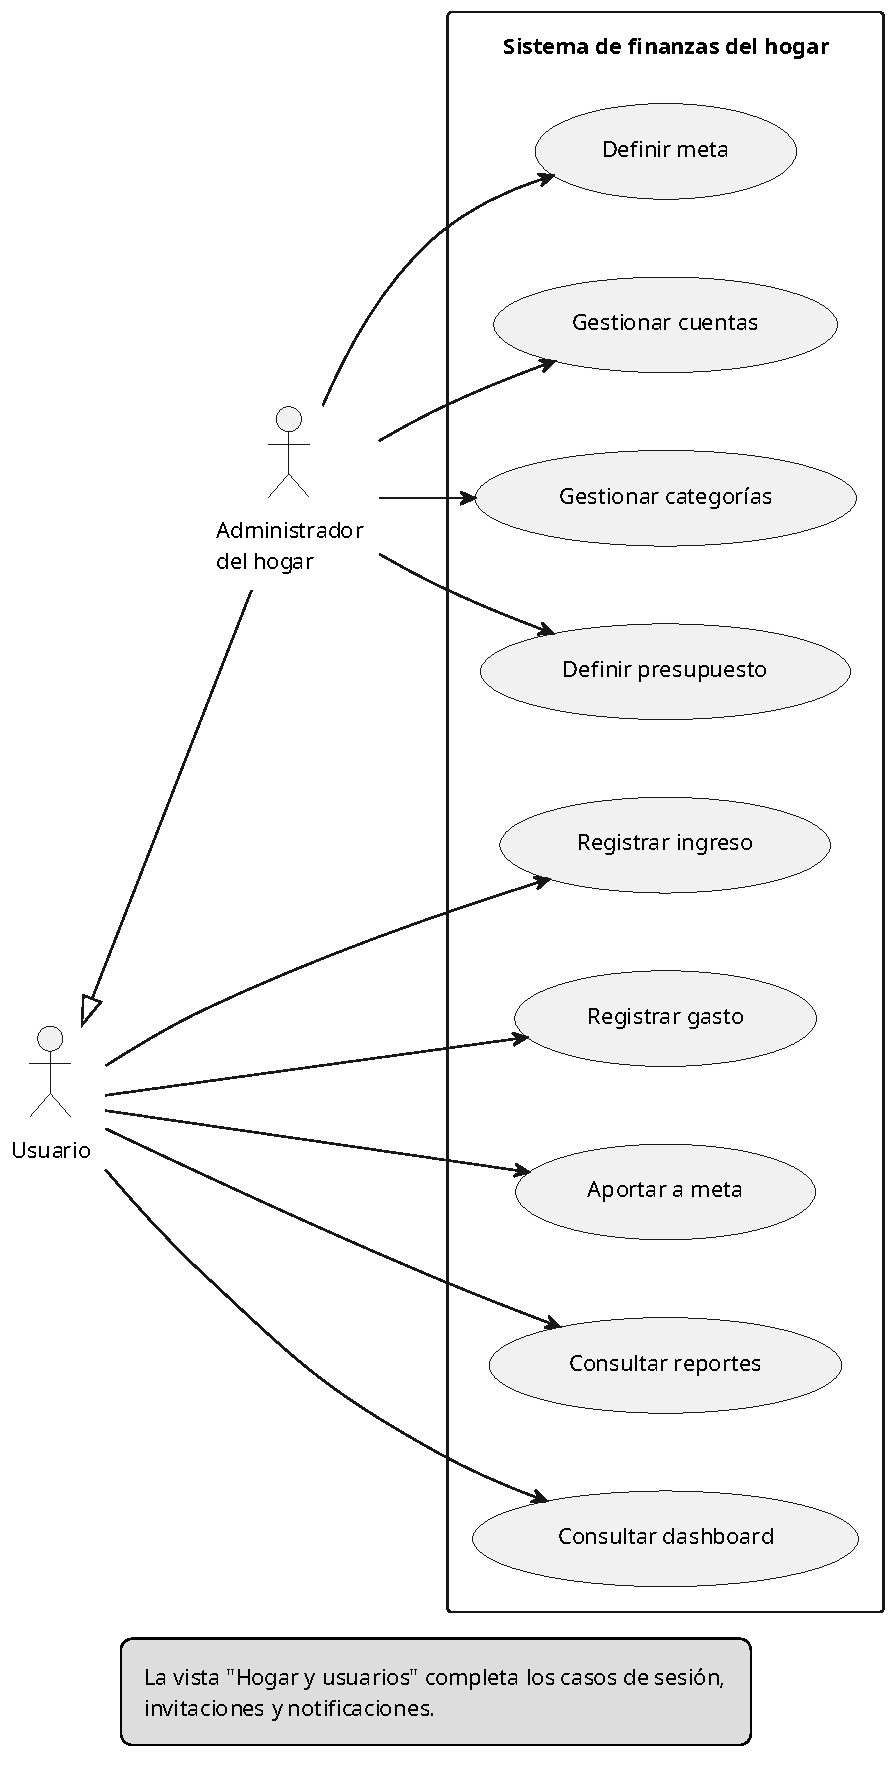
\includegraphics[width=\linewidth]{figuras/pdf/casos-uso-financiero.pdf}
\caption{Operaciones financieras}
\label{fig:casos-uso-financiero}
\end{subfigure}
\begin{subfigure}{0.48\linewidth}
\centering
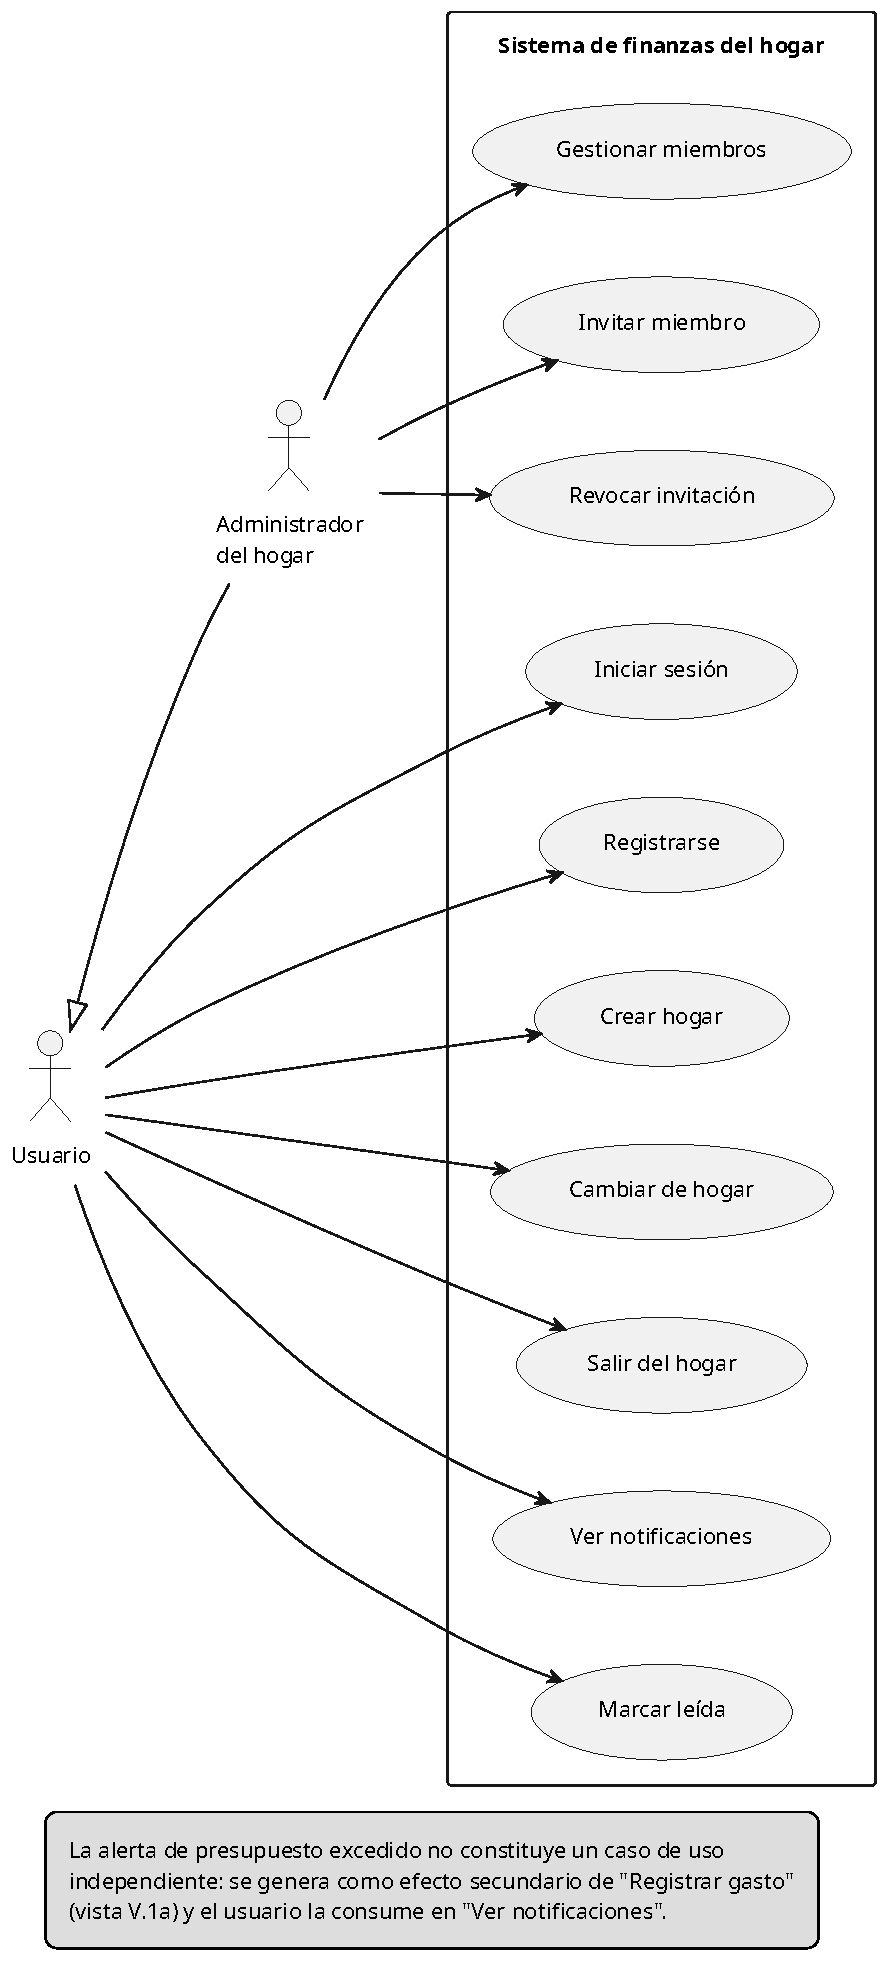
\includegraphics[width=\linewidth]{figuras/pdf/casos-uso-hogar.pdf}
\caption{Hogar y usuarios}
\label{fig:casos-uso-hogar}
\end{subfigure}
\caption{Diagramas de casos de uso del sistema}
\label{fig:casos-uso}
\end{figure*}

\subsubsection{Operaciones financieras}

La Fig.~\ref{fig:casos-uso-financiero} presenta las operaciones que un miembro
del hogar realiza sobre cuentas, categorías, transacciones y presupuestos. Cada
caso de uso corresponde a una acción iniciada por el usuario y delimitada por
el hogar activo. La Fig.~\ref{fig:casos-uso-financiero} evidencia que la
autenticación y la selección de hogar son condiciones previas comunes, no casos
de uso independientes, y que las operaciones de consulta y de escritura
comparten los mismos actores.


\subsubsection{Hogar y usuarios}

La Fig.~\ref{fig:casos-uso-hogar} agrupa las operaciones de registro,
autenticación, gestión de hogares, miembros e invitaciones, junto con la
consulta de notificaciones. Se descartó un actor ``Sistema'' porque los casos
identificados son iniciados por usuarios o por tareas explícitas (envío de
invitaciones), no por procesos autónomos; la alerta de presupuesto se modela
como efecto de ``Registrar gasto'' y se consume en ``Ver notificaciones''. La
Fig.~\ref{fig:casos-uso-hogar} muestra además que la gestión de miembros y la
emisión de invitaciones comparten al administrador del hogar como actor
principal.

\subsection{Diagrama de componentes}

\begin{figure*}[!t]
\centering
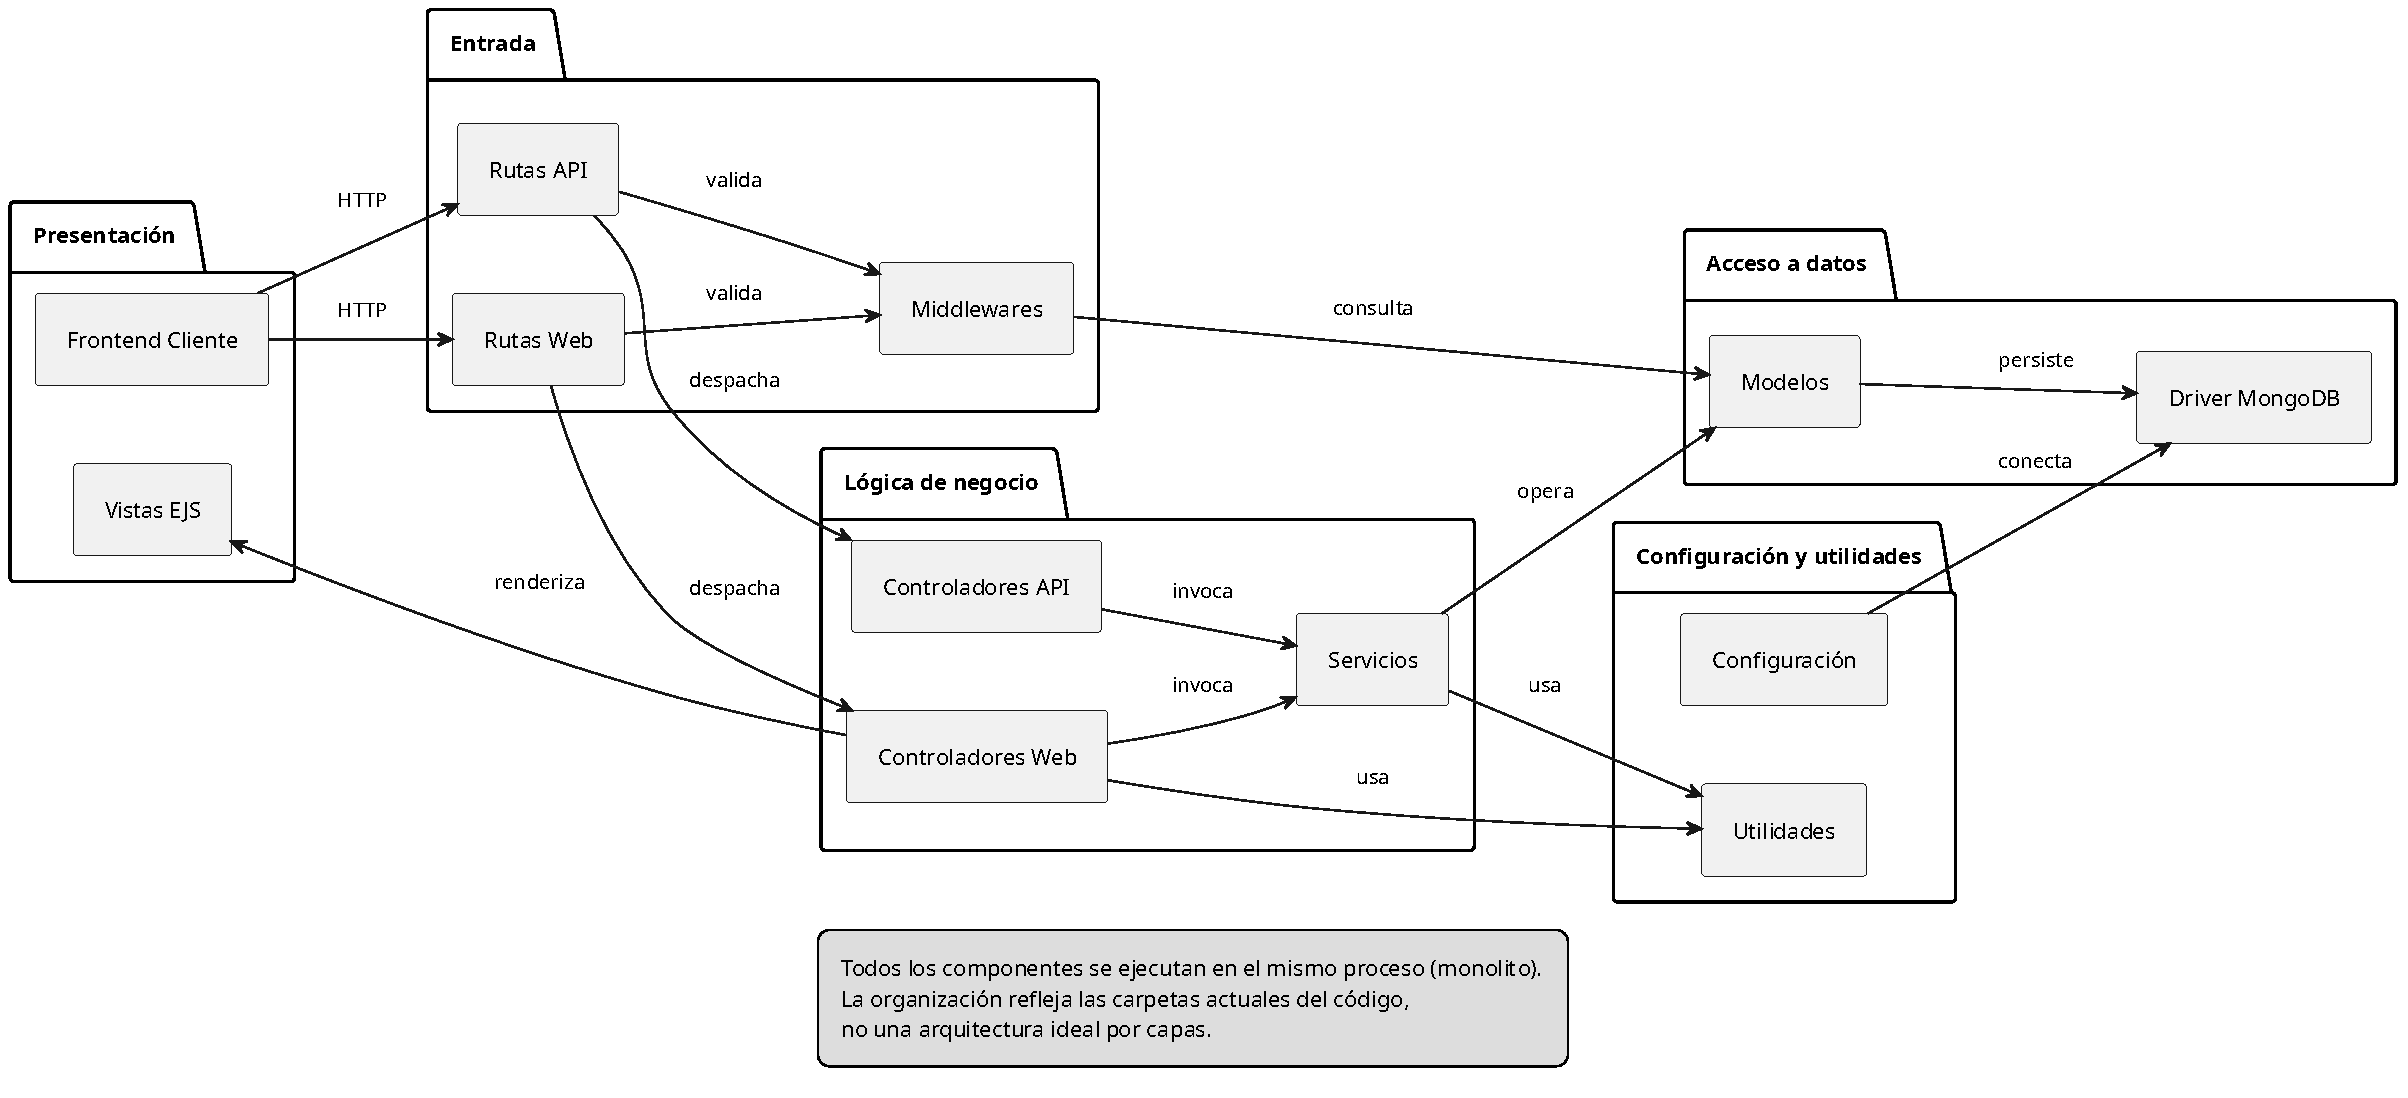
\includegraphics[width=\textwidth]{figuras/pdf/componentes.pdf}
\caption{Componentes y dirección de dependencias}
\label{fig:componentes}
\end{figure*}

La Fig.~\ref{fig:componentes} descompone el sistema en los componentes de
presentación, rutas, controladores, servicios, modelos y persistencia. La
Fig.~\ref{fig:componentes} evidencia que las dependencias apuntan hacia abajo:
las vistas y las rutas conocen a los controladores, los controladores a los
servicios y los servicios a los modelos; ningún componente inferior importa a
uno superior. Esa dirección es la misma que impuso el orden de migración por
capas descrito en la Sección III.


\subsection{Diagrama de secuencia}

\begin{figure*}[!t]
\centering
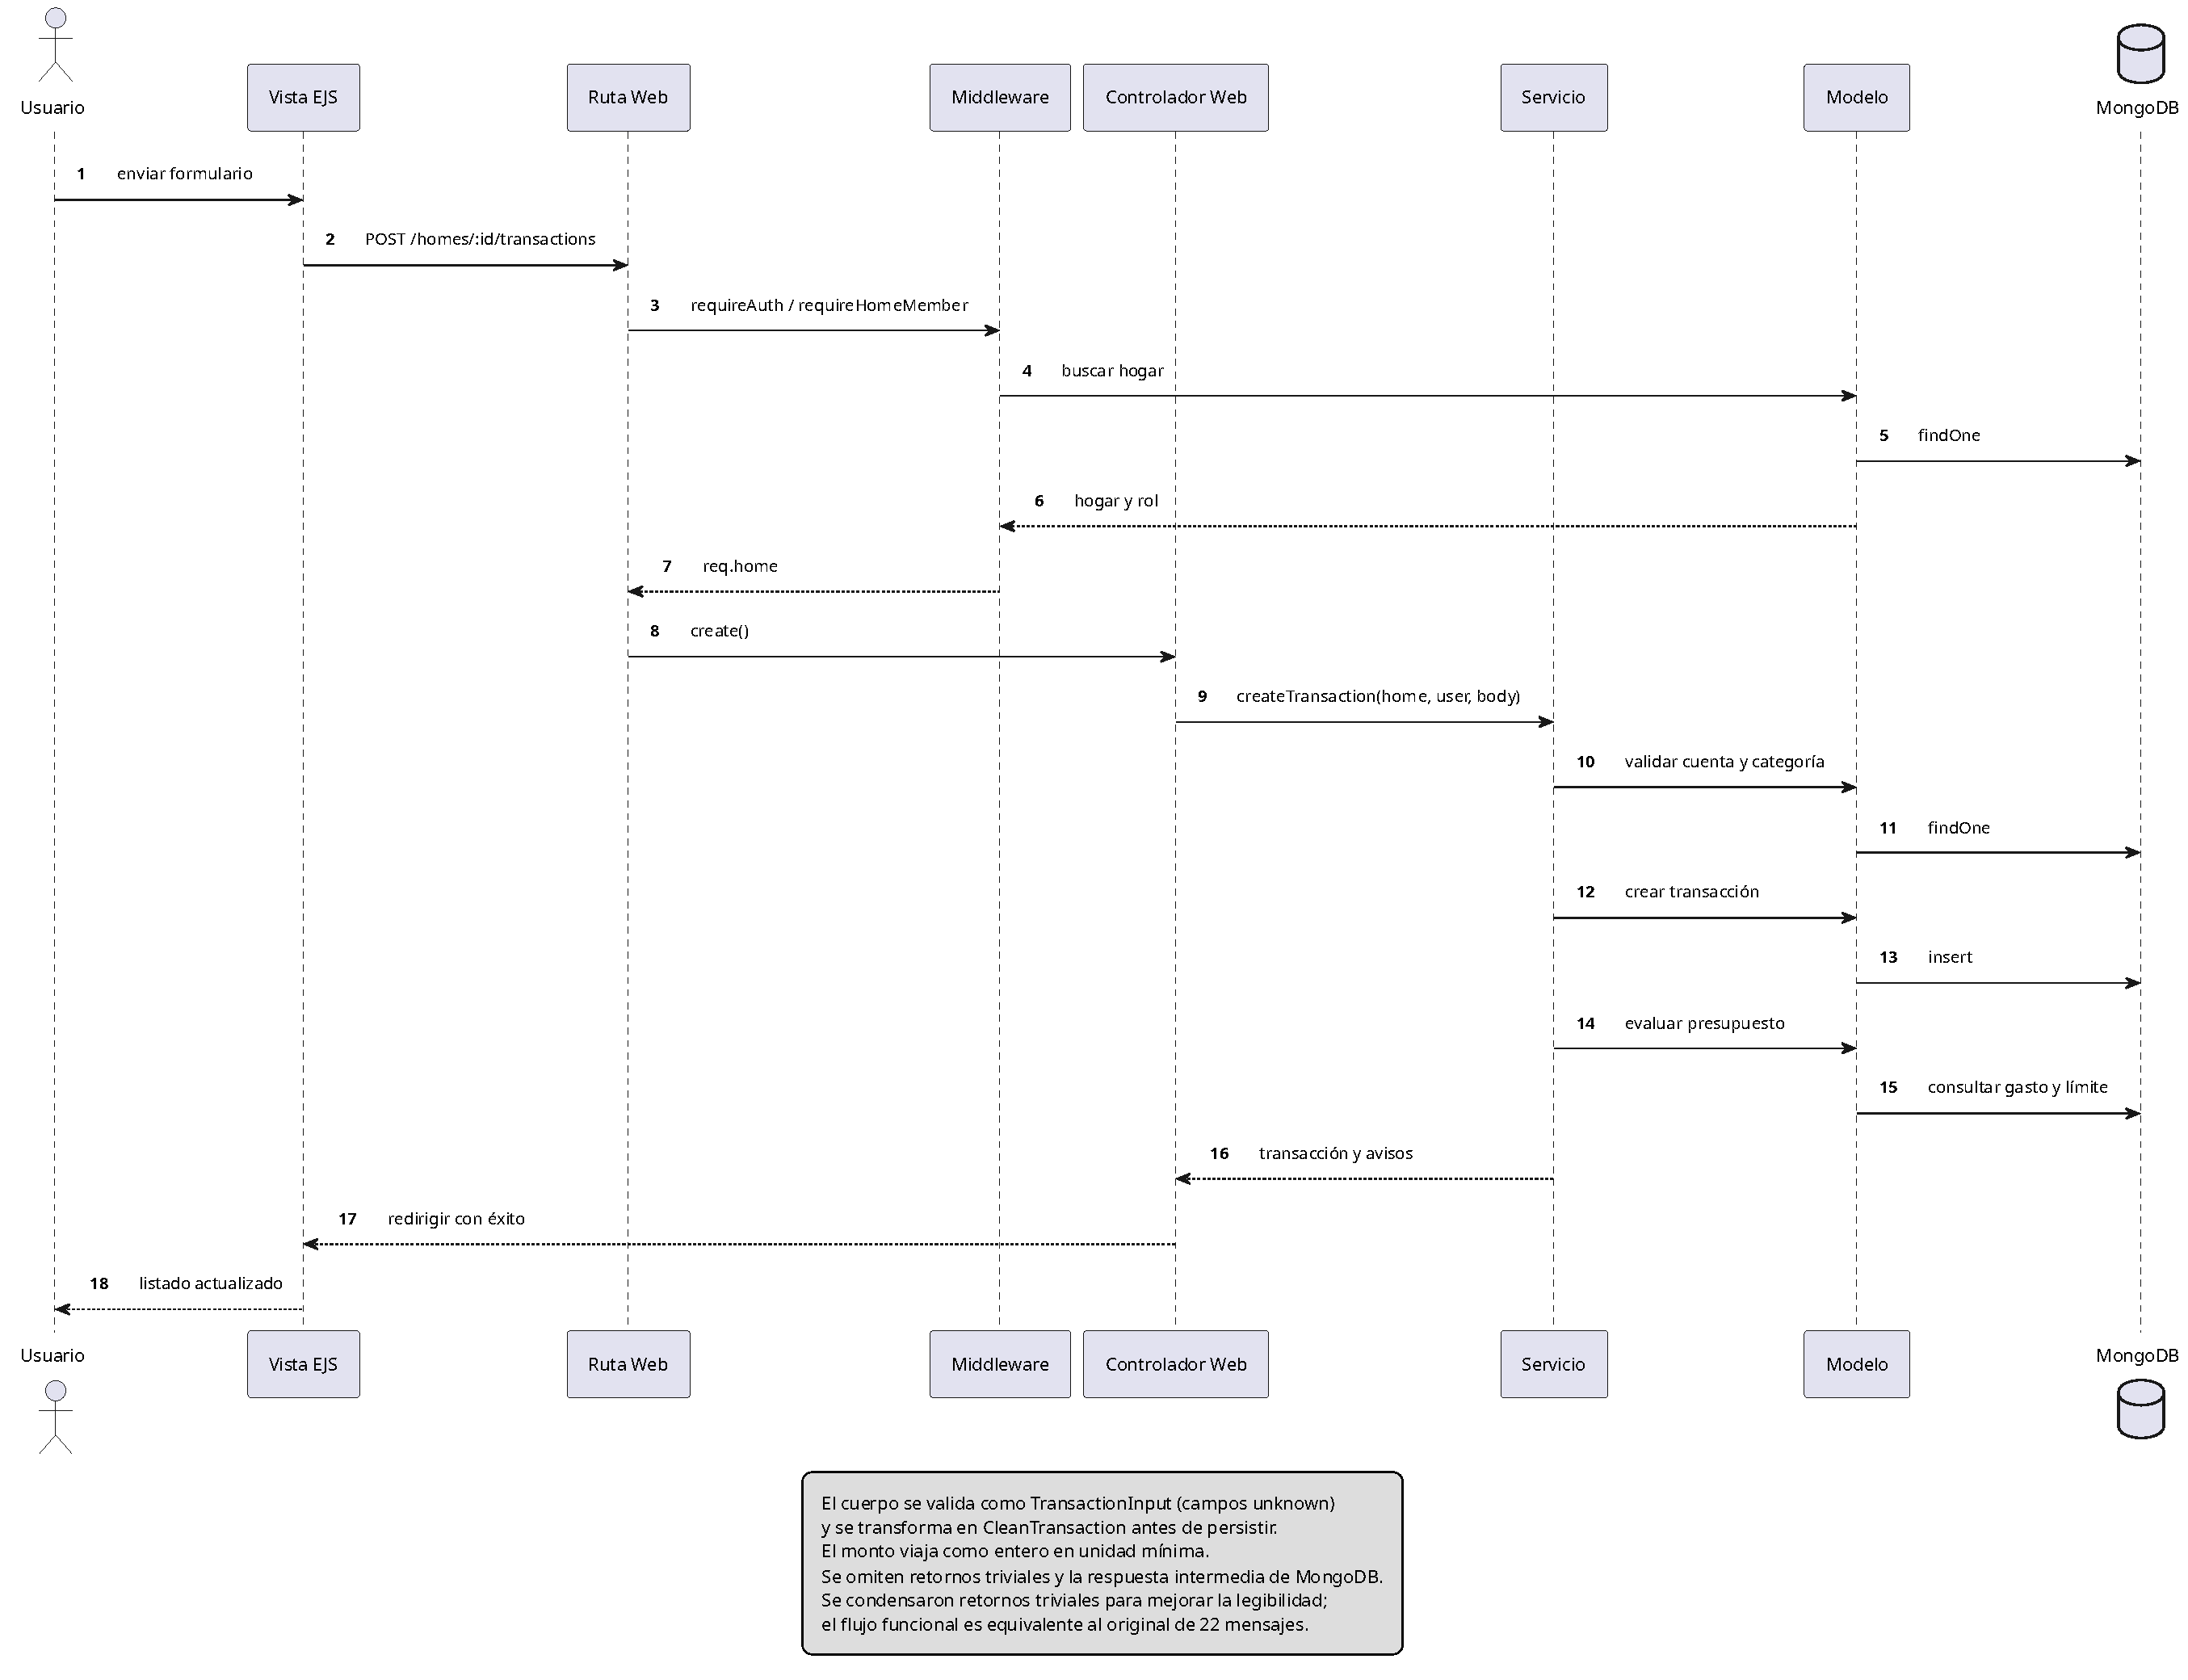
\includegraphics[width=\textwidth]{figuras/pdf/secuencia-registrar-gasto.pdf}
\caption{Secuencia de registro de un gasto. En la versión digital se recomienda
ampliar la figura para leer las etiquetas.}
\label{fig:secuencia}
\end{figure*}

La Fig.~\ref{fig:secuencia} describe el registro de un gasto desde el envío del
formulario hasta la redirección final. La Fig.~\ref{fig:secuencia} evidencia que
la validación de sesión y hogar ocurre antes de invocar al controlador, que el
servicio concentra la creación y la evaluación del presupuesto, y que la
respuesta al usuario no espera a que la notificación se consulte. La secuencia
condensa retornos triviales para mejorar la legibilidad; el flujo funcional es
equivalente al original de 22 mensajes. Para leer las etiquetas en detalle, se
recomienda ampliar la Fig.~\ref{fig:secuencia} en la versión digital.


\subsection{Diagrama de colaboración}

\begin{figure*}[!t]
\centering
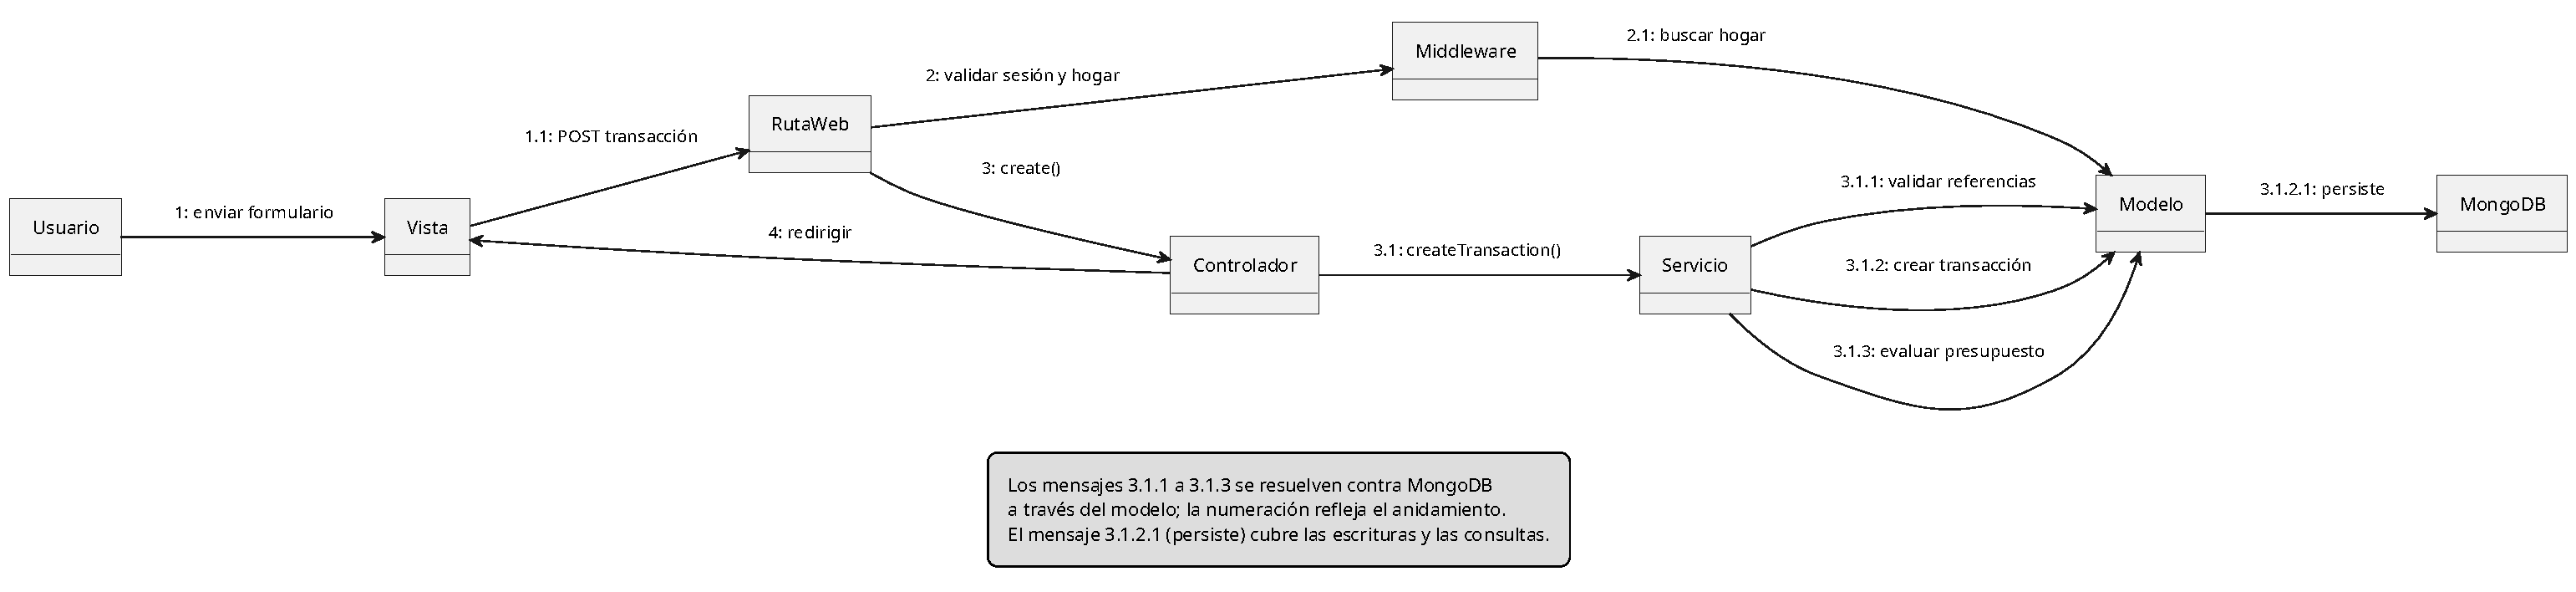
\includegraphics[width=\textwidth]{figuras/pdf/colaboracion-registrar-gasto.pdf}
\caption{Colaboración de objetos en el registro de un gasto. En la versión
digital se recomienda ampliar la figura para leer las etiquetas.}
\label{fig:colaboracion}
\end{figure*}

La Fig.~\ref{fig:colaboracion} presenta la misma operación como una red de
objetos enlazados por mensajes numerados. La Fig.~\ref{fig:colaboracion}
evidencia el anidamiento de las llamadas: el mensaje 3.1.2.1 representa la
persistencia en MongoDB y cubre tanto las consultas como las escrituras que el
modelo resuelve. Los ocho objetos incluyen la base de datos, de modo que la
colaboración no oculta el extremo de persistencia. La lectura de las etiquetas
se facilita ampliando la Fig.~\ref{fig:colaboracion} en la versión digital.


\subsection{Diagramas de clases}
\label{sec:clases}

\begin{figure*}[!t]
\centering
\begin{subfigure}{0.48\linewidth}
\centering
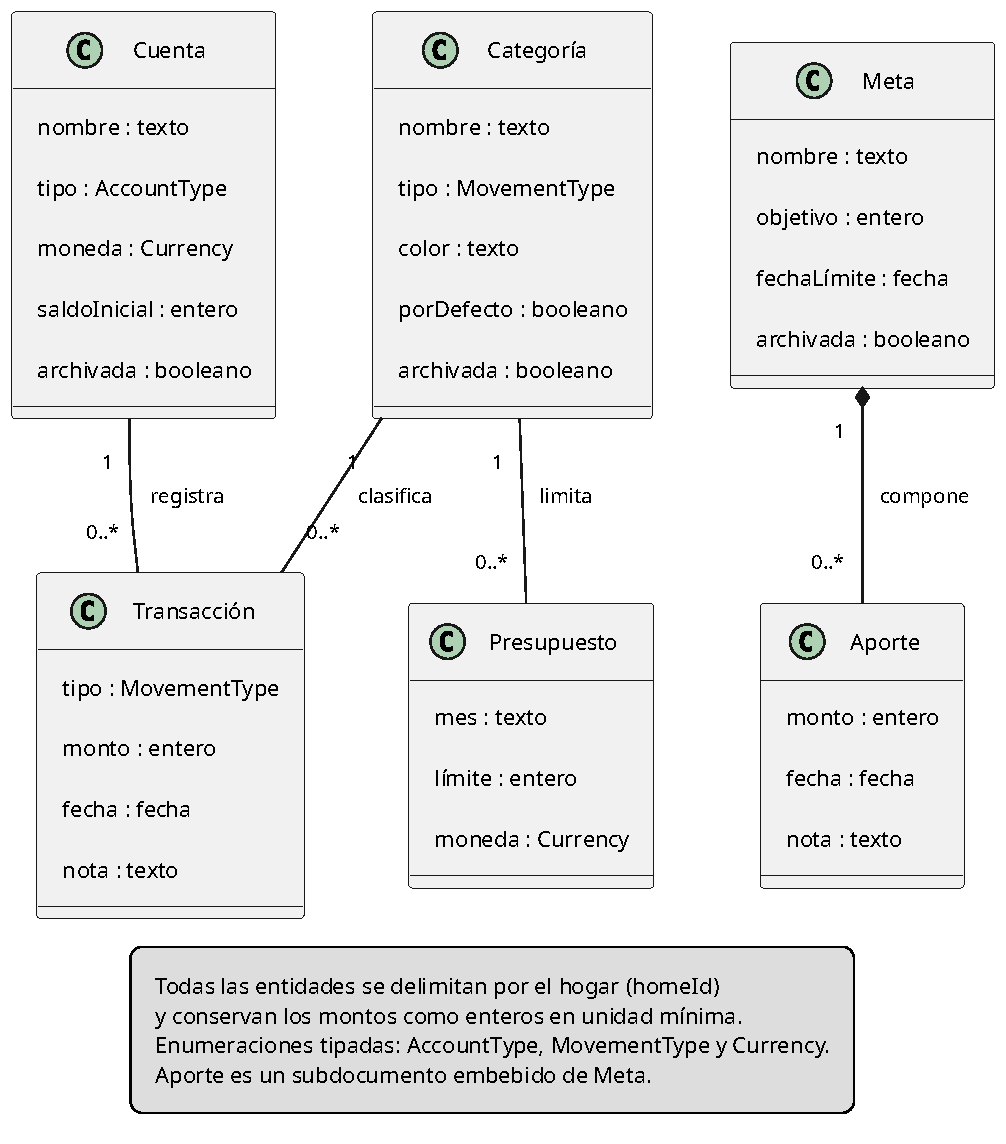
\includegraphics[width=\linewidth]{figuras/pdf/clases-dominio-financiero.pdf}
\caption{Dominio financiero}
\label{fig:clases-financiero}
\end{subfigure}
\begin{subfigure}{0.48\linewidth}
\centering
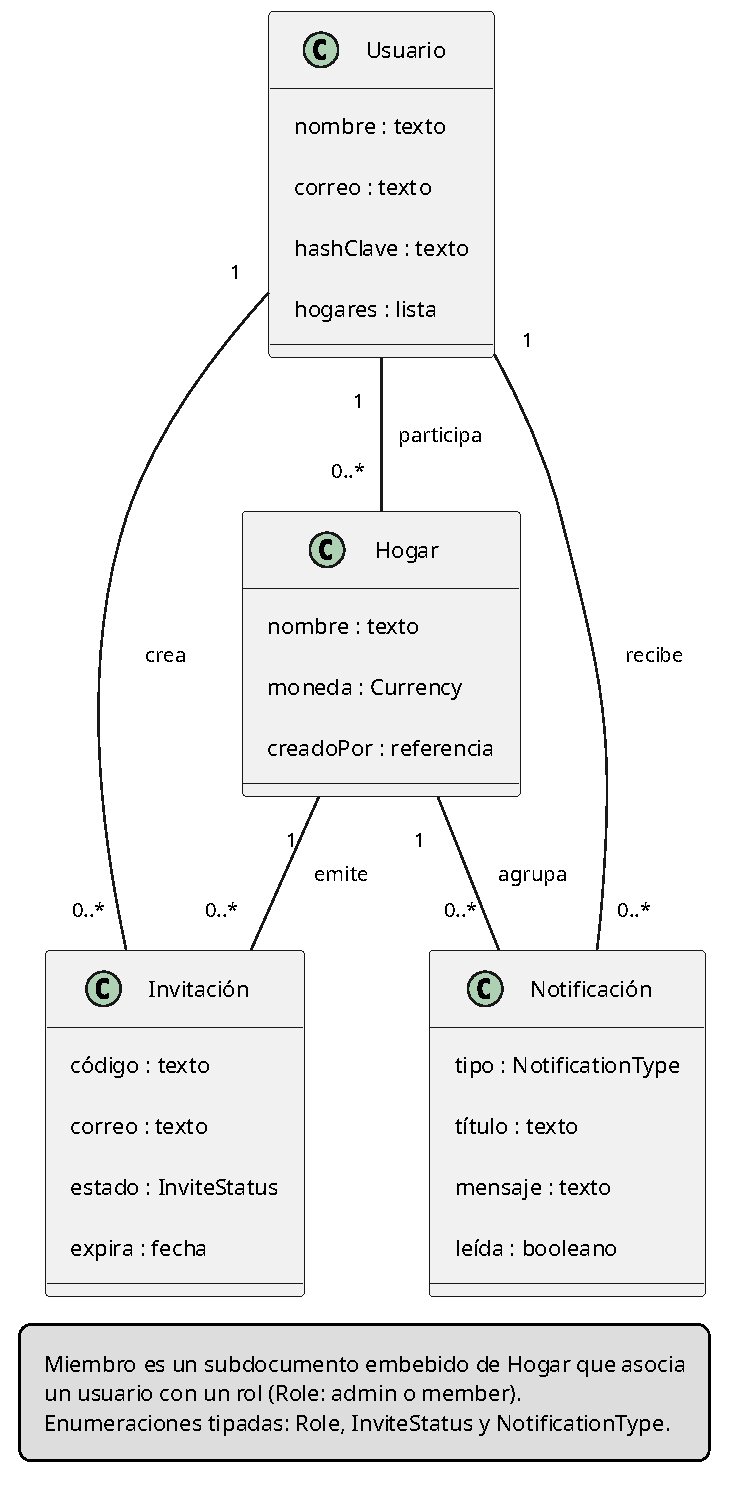
\includegraphics[width=\linewidth]{figuras/pdf/clases-usuarios-hogar.pdf}
\caption{Usuarios y hogar}
\label{fig:clases-usuarios}
\end{subfigure}
\caption{Diagramas de clases del dominio}
\label{fig:clases}
\end{figure*}

\subsubsection{Dominio financiero}

La Fig.~\ref{fig:clases-financiero} reúne las entidades de cuenta, categoría,
transacción, presupuesto, meta y aporte. La Fig.~\ref{fig:clases-financiero}
evidencia que las transacciones referencian una cuenta y una categoría, que los
presupuestos limitan una categoría por mes y que los aportes se componen dentro
de la meta. Las entidades se delimitan por el hogar y conservan los montos como
enteros en la unidad mínima, decisión que evita errores de punto flotante.


\subsubsection{Usuarios y hogar}

La Fig.~\ref{fig:clases-usuarios} presenta las entidades de usuario, hogar,
invitación y notificación. La Fig.~\ref{fig:clases-usuarios} evidencia que la
membresía se modela como un subdocumento del hogar con un rol tipado, que las
invitaciones relacionan al usuario que las crea con el hogar que las emite y
que las notificaciones pertenecen a un usuario y a un hogar. Las
enumeraciones de rol, estado de invitación y tipo de notificación restringen
los valores válidos sin cambiar los datos almacenados.

\section{Resultados, validación y lecciones aprendidas}

\subsection{Resultados de la migración}

Al cierre de la migración, el compilador dejó de emitir diagnósticos sobre el
árbol completo y las suites HTTP quedaron sin fallos. La Tabla~\ref{tab:migracion}
reúne únicamente las cifras de ese momento; no incorpora el conteo de
comprobaciones del estado actual, que se discute en la
Sección~\ref{sec:doble-alcance}. El descenso de 686 a 0 errores de
\texttt{tsc --noEmit} se produjo por capas y sin cambios de comportamiento
observable, y las 204 comprobaciones funcionales se mantuvieron en verde tras
cada cierre de capa.

\begin{table}[!t]
\caption{Resultados al cierre de la migración (commit \texttt{34016bd})}
\label{tab:migracion}
\centering
\small
\begin{tabular}{@{}lcc@{}}
\toprule
Indicador & Antes & Después \\
\midrule
Errores de \texttt{tsc --noEmit} & 686 & 0 \\
Comprobaciones HTTP exitosas & --- & 204/204 \\
Archivos \texttt{.mjs} en \texttt{src/} & 53 & 0 \\
Referencias a \texttt{.mjs} en el código & 106 & 0 \\
\bottomrule
\end{tabular}

\vspace{2pt}
{\footnotesize Fuente: suites HTTP ejecutadas sobre el commit \texttt{34016bd}
(05/11/2026) y \texttt{npm run typecheck} sobre el mismo commit.}
\end{table}

\subsection{Validación funcional}

La validación combinó dos niveles. El primero fue estático: \texttt{npm run
typecheck} ejecuta \texttt{tsc --noEmit} sobre \texttt{src/} y exige cero
diagnósticos. El segundo fue funcional: las suites de HTTP se ejecutaron contra
el servidor iniciado con \texttt{tsx} y la base MongoDB activa. La suite de
estado base preparó usuarios, hogares y sesiones; las suites de transacciones,
presupuestos y permisos, reportes y recursos, y autenticación e interfaz de
programación aportaron 52, 62, 49 y 41 comprobaciones, respectivamente, hasta
sumar 204.

A ello se añadieron comprobaciones puntuales: el documento OpenAPI respondió
con el HTML de Swagger y su archivo de inicialización; las rutas
\texttt{/js/app.js} y \texttt{/js/dashboard.js} sirvieron los paquetes
generados; y el mensaje de sesión se conservó con una sola aparición. La
ausencia de residuos se verificó con dos búsquedas: ninguna extensión
\texttt{.mjs} permaneció bajo \texttt{src/} y ninguna referencia a esa extensión
sobrevivió en \texttt{src/} o \texttt{public/}. Las suites son scripts de shell
alojados en \texttt{.data/tests}; no forman parte de los scripts de
\texttt{package.json} y requieren MongoDB y el servidor en ejecución, por lo que
su reproducción completa depende de ese entorno.

\subsection{Evidencia de snapshots}

La comparación se apoya en ocho pares de archivos reconstruidos desde el
historial: el punto de entrada, el modelo de usuario, el modelo de invitación,
el servicio de cuentas, el middleware de hogar, el controlador de cuentas de la
interfaz de programación, el controlador web de autenticación y la fuente del
frontend. El par de \texttt{src/models/user.ts}, reproducido en el
Listado~\ref{lst:modelo}, es representativo: muestra la interfaz del documento,
la interfaz del contrato y la clase cuyos estáticos se copian con
\texttt{loadClass}. El detalle de los ocho pares y los comandos de comparación
se conserva en el Anexo A.2.

\subsection{Doble alcance temporal}
\label{sec:doble-alcance}

Este artículo distingue dos momentos: el proceso migratorio (cifras 686 a 0 y
204/204, commit \texttt{34016bd}) y el estado actual del repositorio (67
archivos \texttt{.ts}, 577/577 checks en \texttt{cebc62a}). Las cifras actuales
no se contabilizan como resultados de la migración porque corresponden a las
fases A--E posteriores. La distinción es una decisión metodológica: evita
atribuir al proceso migratorio funciones y pruebas que se incorporaron después
de su cierre y permite comparar ambos momentos sin mezclar sus fuentes.

\subsection{Despliegue}

El despliegue en Vercel no ejecuta un paso de compilación: el servidor se inicia
con \texttt{tsx} y el sitio sirve los artefactos ya publicados en
\texttt{public/}. Esa configuración mantiene el typecheck como una verificación
previa y no como un requisito del arranque. La lección de despliegue fue la
resolución de tipos: Vercel instala dependencias con un anidamiento distinto al
local, por lo que \texttt{tsconfig.json} declara \texttt{typeRoots} con las rutas
\texttt{./node\_modules/@types}, \texttt{../node\_modules/@types} y
\texttt{../../node\_modules/@types}. Sin esa declaración, el paquete de tipos de
Node.js no se encontraba en el entorno de ejecución remoto.

\subsection{Lecciones aprendidas}

Tres lecciones resumen el proceso. Primera: en Mongoose, extender una clase
desde \texttt{Model} no aporta tipado porque \texttt{Model} es una interfaz; el
contrato debe declararse como interfaz y los estáticos implementarse en una
clase copiada con \texttt{loadClass}. Segunda: activar \texttt{strict} de forma
incremental por capas convierte el conteo de errores en una señal de avance y
evita mezclar deuda localizada con ruido cruzado. Tercera: separar el typecheck
del build permite verificar el árbol sin generar artefactos y conserva un
despliegue sin paso de compilación.

\section{Conclusiones}

\subsection{Síntesis técnica}

La migración transformó un monolito JavaScript ESM en un árbol TypeScript
estricto sin reescribir la aplicación. El renombrado mecánico, la configuración
del compilador, el orden por capas y la formalización de los modelos permitieron
llegar a cero diagnósticos y mantener 204 comprobaciones funcionales. El patrón
de interfaz de documento, interfaz de modelo y clase de estáticos resolvió el
caso de Mongoose y se generalizó a los nueve modelos actuales.

\subsection{Cumplimiento de objetivos}

Los objetivos se cumplieron con evidencia reproducible: el typecheck desciende
de 686 a 0, las suites cierran en 204/204 y cada par de snapshots queda anclado
a un commit. El valor académico no reside solo en el resultado, sino en el
protocolo: cualquier lector puede repetir el typecheck, ejecutar las suites en
un entorno equivalente y comparar los archivos representativos entre
\texttt{fb1ad1d} y \texttt{34016bd}. La documentación de las decisiones y de las
alternativas descartadas completa esa trazabilidad.

\subsection{Trabajo futuro}

Quedan tres líneas abiertas: incorporar pruebas unitarias sobre servicios y
modelos, añadir una integración continua que ejecute el typecheck en cada
cambio, y versionar el contrato OpenAPI junto con el código para detectar
divergencias entre la documentación y los manejadores. Ninguna de esas líneas
modifica las conclusiones de este artículo.

% Vacía la cola de flotantes antes de la bibliografía.
\clearpage

% Sección VIII: Referencias (IEEEtran genera el encabezado sin numeración).
% Bibliografía gestionada con BibTeX a partir de referencias.bib.
\bibliographystyle{IEEEtran}
\bibliography{referencias}

\section*{Anexo A}
\addcontentsline{toc}{section}{Anexo A}

\subsection*{A.1 Decisiones y alternativas descartadas}

La Tabla~\ref{tab:alternativas} resume las cinco alternativas evaluadas durante
la migración. Todas fueron descartadas por un motivo verificable y sustituidas
por la opción que quedó en el repositorio.

\begin{table}[!t]
\caption{Alternativas descartadas durante la migración}
\label{tab:alternativas}
\centering
\footnotesize
\begin{tabular}{@{}>{\raggedright\arraybackslash}p{1.55cm}>{\raggedright\arraybackslash}p{1.75cm}>{\raggedright\arraybackslash}p{2.0cm}>{\raggedright\arraybackslash}p{2.1cm}@{}}
\toprule
Alternativa & Motivo de descarte & Opción adoptada & Evidencia \\
\midrule
\texttt{class XModel extends Model} & \texttt{Model} es interfaz; colapsa miembros a \texttt{any} & \texttt{IXModel} + clase con \texttt{loadClass} & \texttt{models/\allowbreak user.ts} \\
\texttt{tsc} + ejecución de \texttt{dist/} & Añade build al despliegue; Vercel no lo ejecuta & \texttt{tsx} en runtime + \texttt{tsc --noEmit} & \texttt{package.json} \\
\texttt{catch (err: any)} & Anula el chequeo estricto del error & \texttt{unknown} + \texttt{isHttpError} & \texttt{middlewares/\allowbreak error.ts} \\
Guardia de hogar por ruta & Duplica control y altera flujos de error & Aserción no nula tras el middleware & \texttt{types/\allowbreak express.d.ts} \\
Frontend sin migrar & Mantiene dos lenguajes y contratos distintos & TypeScript + esbuild con artefactos versionados & \texttt{package.json} (\texttt{build:ui}) \\
\bottomrule
\end{tabular}

\vspace{2pt}
{\footnotesize Fuente: repositorio en el commit \texttt{34016bd} (05/11/2026)
y sección 11 del documento de migración.}
\end{table}

\subsection*{A.2 Trazabilidad de snapshots}

Los archivos de \texttt{antes/} provienen del commit \texttt{fb1ad1d}, estado
previo a la migración. Los de \texttt{despues/} provienen del commit
\texttt{34016bd} (``Migración completa a TypeScript estricto''), que cierra la
migración, y no de \texttt{HEAD}. El estado actual del repositorio puede
diferir de estos snapshots por las fases posteriores A--E. La
Tabla~\ref{tab:snapshots} enumera los ocho pares reconstruidos.

\begin{table}[!t]
\caption{Pares de snapshots reconstruidos entre \texttt{fb1ad1d} y \texttt{34016bd}}
\label{tab:snapshots}
\centering
\footnotesize
\begin{tabular}{@{}>{\raggedright\arraybackslash}p{4.2cm}>{\raggedright\arraybackslash}p{3.8cm}@{}}
\toprule
Par (antes $\rightarrow$ después) & Aspecto diferencial \\
\midrule
\texttt{app.mjs} $\rightarrow$ \texttt{app.ts} & Punto de entrada, locales y doble arranque \\
\texttt{models/user.mjs} $\rightarrow$ \texttt{models/user.ts} & Interfaz, clase y estáticos \\
\texttt{models/invite.mjs} $\rightarrow$ \texttt{models/invite.ts} & Enumeraciones tipadas \\
\texttt{accountService.mjs} $\rightarrow$ \texttt{.ts} & Entradas tipadas y errores \\
\texttt{middlewares/home.mjs} $\rightarrow$ \texttt{home.ts} & Augmentación de la petición \\
\texttt{api/accountController.mjs} $\rightarrow$ \texttt{.ts} & Manejadores tipados \\
\texttt{web/authController.mjs} $\rightarrow$ \texttt{.ts} & Cuerpos y flujos web \\
\texttt{public/js/app.js} $\rightarrow$ \texttt{src/frontend/app.ts} & DOM tipado y bundle \\
\bottomrule
\end{tabular}

\vspace{2pt}
{\footnotesize Fuente: \texttt{INDICE.md} de la carpeta de snapshots; commit de origen
\texttt{fb1ad1d} y commit de destino \texttt{34016bd} (05/11/2026).}
\end{table}

La comparación de un par se reproduce desde el directorio
\texttt{snapshots-migracion/} con los comandos siguientes:

{\ttfamily\scriptsize
\noindent\verb|diff -u antes/src/models/user.mjs despues/src/models/user.ts|\\
\noindent\verb|diff -u antes/src/app.mjs despues/src/app.ts|
\par}

Los Listados 1 y 3 no forman parte de los ocho snapshots: \texttt{tsconfig.json}
y \texttt{src/types/express.d.ts} se citan directamente desde el commit
\texttt{34016bd}, como se indica en sus notas al pie. Para reproducir el parche
de fuentes de la plantilla IEEEtran, el comando exacto es:

{\ttfamily\scriptsize
\noindent\verb|sed -i '495s/{ptm}/{cmr}/' \|\\
\noindent\verb|  texmf/tex/latex/ieeetran/IEEEtran.cls|\\
\noindent\verb|sed -i '4595s/{ptm}/{cmr}/' \|\\
\noindent\verb|  texmf/tex/latex/ieeetran/IEEEtran.cls|
\par}

\end{document}
